% !TeX encoding = UTF-8
% !TeX program = XeLaTeX
% !TeX spellcheck = en_US

\documentclass[english]{../TexTemplate/thesis}
\usepackage{../TexTemplate/mypackage}
\usepackage{ctex}

\linespread{1.25}

\title{Week 5 - Python Basics}
\author{Hongzheng Chen}
\date{Dec 13, 2019}
\headercontext{Week 5 - Python Basics}

\begin{document}

\maketitle

\section{Installation and Configuration}
Unix-like systems basically pre-install Python distribution, which can be easily called by \verb'python' or \verb'python3'.
If your Python version is 2.x, please update to 3.x, since Python organization will no longer support 2.x when it comes to 2020.

\href{https://www.jetbrains.com/pycharm/}{PyCharm} is the widely used IDE for Python, but I am \textbf{not} recommend you to install, since VS Code has had initial support for Python and its extensions, which performs well and gets much better and better in recent versions.
If you use Windows and Linux dual system (including those using WSL), what I recommend is to install \href{https://www.anaconda.com/}{Anaconda}, an extremely powerful platform for Python development. The build-in \href{https://conda.io/en/latest/}{conda} and \href{https://pypi.org/project/pip/}{pip} management tools make Python packages in order, and many packages (like \href{https://pytorch.org/}{pytorch} for deep learning) can only be installed in this way. Detailed usage of Anaconda will be covered in the next few seminars, so you only need to download and install it.

If you use a singleton Unix-like system (e.g. MacOS, Linux whole system), everything is easy. No need for Anaconda. Once \href{https://pypi.org/project/pip/}{pip} is installed, you get rid of tedious configuration steps for different packages.

\section{Resources}
There are massive Python tutorials on the Chinese Internet, and you can easily find them on Zhihu or Baidu, but most of them are not systematic enough.
Thus, several recommended introductory materials are listed here:
\begin{itemize}
	\item \emph{Learning Python: Powerful Object-Oriented Programming} (Chinese: \href{https://item.jd.com/12452929.html}{《Python学习手册》}): The slide's examples are based on this book, and the electronic version can be found on net disk. This book is very long but extremely detailed. It is highly recommended to get through all its chapters and compare Python with C/C++. If you are familiar with C++, these contents can be learned quickly. But if you are still struggling with C/C++, learn \emph{C++ Primer} first.
	\item \emph{Structure and Interpretation of Computer Programs} (SICP, Python version): This book is firstly written in Scheme but latter translated into Python and becomes the introductory course of University of Berkeley, i.e. \href{https://cs61a.org/}{UCB 61A}.
	Prof. Xinyu Feng in Nanjing University introduces it to China, his course can be found on \href{https://cs.nju.edu.cn/xyfeng/teaching/SICP/}{NJU 22000130}.
	\item \emph{Python Crash Course: A Hands-On, Project-Based Introduction to Programming} (Chinese: \href{https://item.jd.com/11993134.html}{《Python编程:从入门到实践》}): It gives several application projects in the last few chapters. This book can be found on net disk.
	\item Official \href{https://docs.python.org/3.6/}{Python 3.6 documentation}: using it as a manual is the best way.
	\item \href{https://www.shiyanlou.com/courses/596}{实验楼 - \emph{Python3 简明教程}}: You can use its interactive environment to learn Python, which is very down-to-earth. But maybe it is time-consuming if you have basic knowledge of programming languages.
	\item \emph{\href{https://www.liaoxuefeng.com/wiki/1016959663602400}{廖雪峰 - Python教程}}: concise but may miss some details.
\end{itemize}

You should read through \href{https://www.python.org/dev/peps/pep-0008/}{PEP 8} (\emph{Style Guide for Python code}) and \href{https://www.python.org/dev/peps/pep-0020/}{PEP 20}, and remember them in mind when you coding.

Moreover, Python will be used through the following seminars, your courses in sophomore and junior, and maybe your whole career life.
Therefore, learn it carefully and get as deep as you can.

\section{Project}
\textbf{Use Python to implement a Python interpreter.}
The flow of interpreter is shown in Fig.~\ref{fig:flow}.
Detailed descriptions will be posted later.

\begin{figure}[H]
\centering
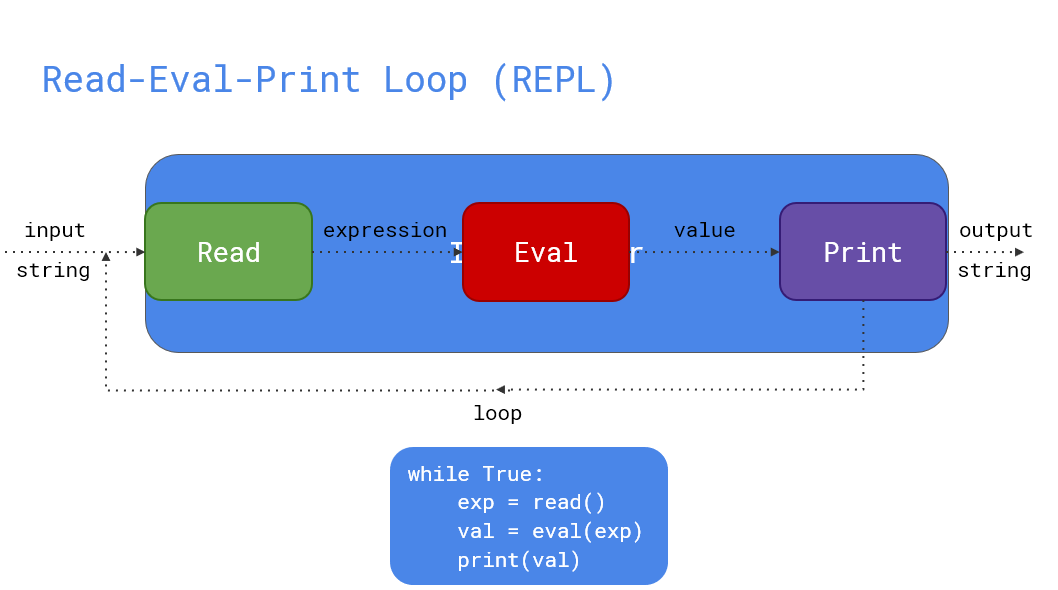
\includegraphics[width=0.8\linewidth]{fig/repl.png}
\caption{A basic interpreter flow: Read-Eval-Print Loop (REPL)}
\label{fig:flow}
\end{figure}

Some reference materials:
\begin{itemize}
	\item \href{https://github.com/aosabook/500lines/tree/master/interpreter}{Byterun}: A 500-line-code Python-based Python interpreter, which is based on \href{https://en.wikipedia.org/wiki/Stack_machine}{Stack machine} and may be very slow. Its description can be found in this \href{http://qingyunha.github.io/taotao/}{Chinese blog}.
	\item \href{https://pypy.org/}{PyPy}: A Python-implemented \href{https://en.wikipedia.org/wiki/Just-in-time_compilation}{Just-in-time (JIT)} Python compiler. It is much faster than the official CPython implementation in some specific cases.
	\item \href{https://cs.nju.edu.cn/xyfeng/teaching/SICP/lectureNotes/20-Interpreters.pptx}{NJU SICP} 20 - Interpreters: This slide gives the basic knowledge of interpreters.
\end{itemize}

\end{document}